% !TEX root = ../Thesis.tex
\chapter{Mathematical tools}
\section{Power Iterations}
\label{sec:powerIterations}

Power iteration (also called power method) is a iteratively method, 
which approximates the biggest eigenvalue of a diagonalizable matrix $A$.

The algorithm starts with a random vector $b_0$ or an approximation of the dominant eigenvector.

\begin{equation}
    \label{eq:powerIterations}
    b_{k+1} = \frac{Ab_k}{||Ab_k||}
\end{equation}

\textbf{TODO:convergence if there is only one largest eigenvalue and if b0 is not orthogonal to the eigenvector associated with the largest eigenvalue.}

The algorithm not necessarily converges. The algorithm will converge, if $A$ has an eigenvalue strictly grater than its other eigenvalues
and the initial vector $b_0$ has a component in direction of an eigenvector, associated with the dominant eigenvector.

\section{Folded spectrum Method}

\textbf{TODO: I don't know what is the Hamiltonian matrix, so either you define it or don't talk about it. 
You can also introduce the folded spectrum just as a way to recover the eigenvector associated with a known eigenvalue. Epsilon often refers to a very small scalar.}


\label{sec:FoldedSpectrumMethod}
Calculation of eigenvalues and eigenvectors of a given Hamiltonian matrix $H$ 
is a fundamental mathematical problem. Often, we are interested in just the smallest 
values, which can be efficiently computed. But if we are interested in selected values,
this can be hard. $H$ is needed to be diagonalized (bring matrix $H$ into diagonal form) 
which is computationally expensive and for big matrices impossible.

Currently, the best way to solve such problems is the Folded spectrum (FS)\cite{foldedSpectrumMethod} method,
which iteratively solves the problem. During calculation, the eigenvalue spectrum will be folded around a reference 
value $\epsilon$.

\begin{equation}
    \label{eq:foldedSpectrumMethod}
    v^{t+1} = v^t - \alpha (H - \epsilon I )^2 v^t ,
\end{equation}

with $0 < \alpha < 1$. When $t \rightarrow \infty$, then $v^{\infty}$ will be the 
eigenvector with respect to the reference value $\epsilon$.


\section{Wasserstein metric}
\label{sec:wasserstein-metric}
\textbf{TODO: the difference between Wasserstein and KL divergence for instance is that it is defined (the value is finite) even if the two distributions have not the same support. }


The Wasserstein metric is a distance measure between two probability distributions and it is used in ML as a loss function\cite{learningWithWasserstein}. 
Intuitively, it can can be understood as the minimum cost to transfer the mass of one distribution to the other.
Therefore, it is also known as the \textit{earth mover's distance}.

As \citet{wassersteinGAN} could show, ordinary distance measures like \textit{Total Variation}, \textit{Kullback-Leibler divergence}
and \textit{Jensen-Shannon divergence} are not sensible when learning with distributions supported by manifolds
On the contrary, Wasserstein metric does a good job as loss function in such scenarios.


\section{Fourier Transform}
\textit{Fourier Analysis} is the overall field of study, which deals with representing (or approximating) functions as 
sums of trigonometric functions. When the function is defined in such a way, we are talking from the \textit{Fourier Domain}.

\textit{Fourier transform} (FT) is the way of transforming signals to the Fourier Domain, which is popular in ML.
Basically, with the Fourier transform, a signal can be decomposed to a \textit{Fourier series}, which consists of many weighted sinusoids. 

\paragraph{Fourier-slice theorem}
The Fourier-slice theorem \cite{fourierSliceTheorem} in 3D is defined as follows:

\begin{equation}
    \label{eq:Fourrier-slice}
    F_2 P_2 = S_2 F_3,
\end{equation}

where $F2$ and $F3$ are FTs in 2D and 3D respectively, P2 is a projection operator ($P_2 : 3D \rightarrow 2D$) and $S2$ is the restriction operator.

As pointed out by \cite{cryoEmMath},
the Fourier-slice theorem is the foundation of the reconstruction problem in computerized tomography (CT), which will be explained in section~\ref{sec:reconstructionProblemCT}.
It states, that the 2D FT of the tomographic projection is the same as the 3D FT restricted to a 2D plane through the origin.
Basically, for the CT reconstruction problem, acquiring samples from known viewing directions is the same 
as sampling the 3D Fourier-space. This concept is exploited by the filter BackProjection algorithms, see section~\ref{sec:filterBackProjection}.

\section{Radon Transform}
The radon transform\cite{radonTransform} is the main mathematically concept of tomographic reconstruction.

It is an integral transformation of a function $f(x,y)$, which is defined on the plane. In tomographic reconstruction
the function $f$ will be the observed tomographic image.
The radon transform then transforms $f$ to a function $Rf$, which corresponds to the line integral of the line defined by 
the two parameters $\theta$ and $s$, where $\theta$ is a angle and $s$ the distance to the origin.

In Figure~\ref{fig:phantom_theta45} and Figure~\ref{fig:phantom_theta45_s14} on can see two plots of different
values for $\theta$ and $s$, where $f(x,y)$ is the Shepp-Logan phantom. The complete $Rf(\theta=45, s=0)$, 
which is also called \textit{sinogram}, can be see in Figure~\ref{fig:phantom_sinogram}

\begin{figure}[H]
    \centering
    \subbottom[Radon Transform  $R f(\theta=45, s=0)$\label{fig:phantom_theta45}]{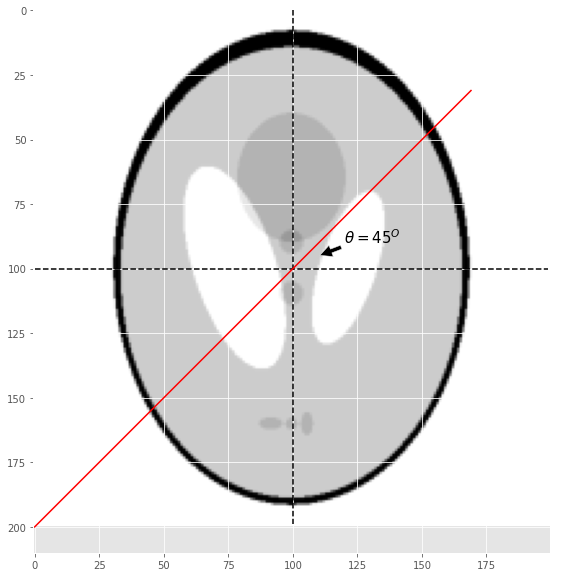
\includegraphics[width=0.3\textwidth]{phantom_theta45.png}}
    \subbottom[Radon Transform  $R f(\theta=45, s=14.14)$\label{fig:phantom_theta45_s14}]{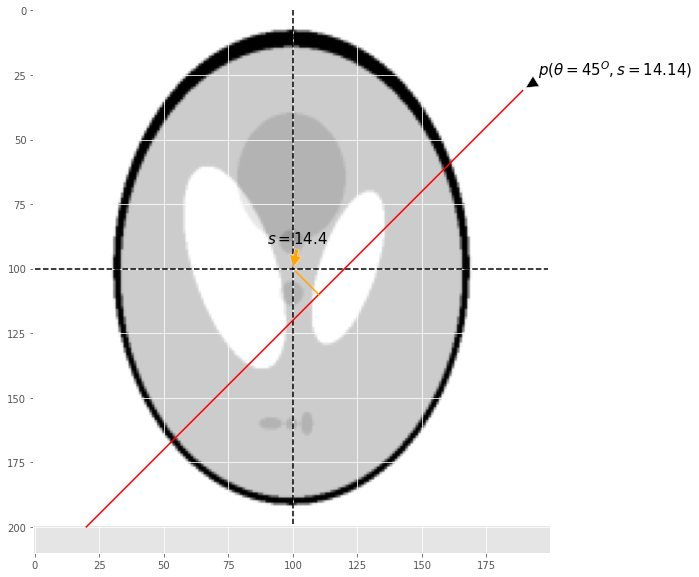
\includegraphics[width=0.3\textwidth]{phantom_theta45_s14.png}}
    \subbottom[Shepp–Logan phantom sinogram of $Rf(\theta=45, s=0)$\label{fig:phantom_sinogram}]{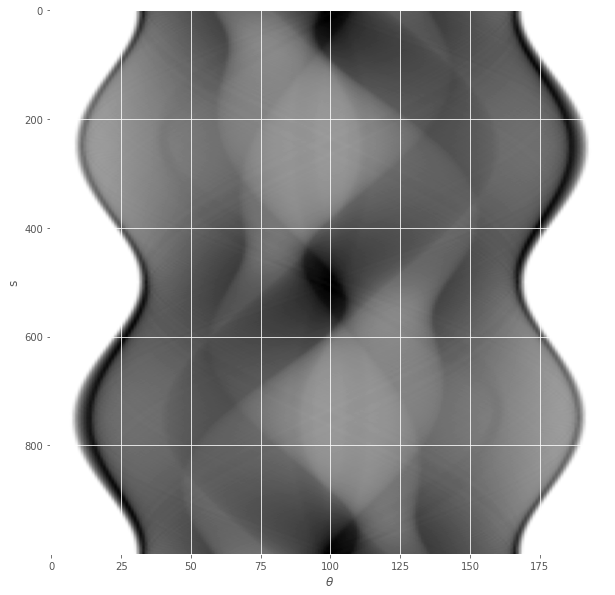
\includegraphics[width=0.3\textwidth]{phantom_sinogram.png}}
    \caption{Examples, where the original object $x$ is the Shepp-Logan phantom.}
\end{figure}